\documentclass{beamer}
\usepackage[utf8]{inputenc}

\usetheme{Madrid}
\usecolortheme{default}
\usepackage{txfonts}
\usepackage{listings}
\usepackage{adjustbox}
\usepackage{tabularx}
\usepackage{lmodern}
\usepackage{circuitikz}
\usepackage{tikz}

\usepackage{gvv}
\usepackage{cite}
\usepackage{amsmath,amssymb,amsfonts,amsthm}
\usepackage{algorithmic}
\usepackage{graphicx}
\usepackage{textcomp}
\usepackage{xcolor}
\usepackage{txfonts}
\usepackage{listings}
\usepackage{enumitem}
\usepackage{mathtools}
\usepackage{gensymb}
\usepackage{comment}
\usepackage{tkz-euclide} 
\usepackage{listings}                                      
\def\inputGnumericTable{}                                
\usepackage{color}                                            
\usepackage{array}                                            
\usepackage{longtable}
\usepackage{multicol}
\usepackage{calc}                                             
\usepackage{multirow}                                         
\usepackage{hhline}                                           
\usepackage{ifthen}

\setbeamertemplate{page number in head/foot}[totalframenumber]

\usepackage{tcolorbox}
\tcbuselibrary{minted,breakable,xparse,skins}



\definecolor{bg}{gray}{0.95}
\DeclareTCBListing{mintedbox}{O{}m!O{}}{%
  breakable=true,
  listing engine=minted,
  listing only,
  minted language=#2,
  minted style=default,
  minted options={%
    linenos,
    gobble=0,
    breaklines=true,
    breakafter=,,
    fontsize=\small,
    numbersep=8pt,
    #1},
  boxsep=0pt,
  left skip=0pt,
  right skip=0pt,
  left=25pt,
  right=0pt,
  top=3pt,
  bottom=3pt,
  arc=5pt,
  leftrule=0pt,
  rightrule=0pt,
  bottomrule=2pt,
  toprule=2pt,
  colback=bg,
  colframe=orange!70,
  enhanced,
  overlay={
    \begin{tcbclipinterior}
    \fill[orange!20!white] (frame.south west) rectangle ([xshift=20pt]frame.north west);
    \end{tcbclipinterior}},
  #3,
}
\lstset{
    language=C,
    basicstyle=\ttfamily\small,
    keywordstyle=\color{blue},
    stringstyle=\color{orange},
    commentstyle=\color{green!60!black},
    numbers=left,
    numberstyle=\tiny\color{gray},
    breaklines=true,
    showstringspaces=false,
}

\title 
{1.9.20}
\date{September 5, 2025}


\author 
{Sai Sreevallabh - EE25BTECH11031}



\begin{document}


\frame{\titlepage}
\begin{frame}{Question}
Find the point on the Y-Axis which is equidistant from the points $\brak{5,-2}$ and $\brak{-3,2}$.
\end{frame}



\begin{frame}{Theoretical Solution}

Given points are\\
\begin{align}
    \vec{A}=\myvec{5\\-2} \ \text{and}\  \vec{B}=\myvec{-3\\2}
\end{align}

Let $\vec{P}$ be a point on the Y-Axis. \\
\begin{align}
    \vec{P}=\myvec{0\\y}
\end{align}

\end{frame}


\begin{frame}{Theoretical Solution}

$\vec{P}$ is equidistant from both $\vec{A}$ and $\vec{B}$. Hence the norms of vectors $\vec{P}-\vec{B}$ and $\vec{P}-\vec{A}$ are equal. 

\begin{align}
    \norm{\vec{P}-\vec{B}} =& \norm{\vec{P}-\vec{A}}\\
    \implies  \norm{\vec{P}-\vec{B}}^2 =& \norm{\vec{P}-\vec{A}}^2\\
    \implies \norm{\vec{P}}^2 - 2\vec{P}^\top\vec{A} + \vec{A}^2 =& \norm{\vec{P}}^2 - 2\vec{P}^\top\vec{B} + \vec{B}^2
\end{align}

\end{frame}

\begin{frame}{Theoretical Solution}

Simplification of the above results in:
\begin{align}
    \brak{\vec{A}-\vec{B}}^\top\vec{P} = \frac{\norm{A}^2 - \norm{B}^2}{2} 
\end{align}

\begin{align}
    \because \vec{P} = y\vec{e_2}   
\end{align}

% \hfill{where, $\vec{e_2} = \myvec{0\\1}$.}          

\begin{align}
    y = \frac{\norm{A}^2-\norm{B}^2}{2\brak{\vec{A}-\vec{B}}^\top\vec{e_2}}
\end{align}

\end{frame}

\begin{frame}{Theoretical Solution}
Substituting the values of $\vec{A}$ and $\vec{B}$:

\begin{align}
    y = \frac{\norm{\myvec{5\\-2}}^2 - \norm{\myvec{-3 \\2}}^2}{2\myvec{8 & -4}\myvec{0\\1}}
\end{align}

\begin{align}
    y = -2
\end{align}

$\therefore$ The point on the y-axis that is equidistant from the given two points is $\vec{P}$ = $\myvec{0\\-2}$.

\end{frame}

\begin{frame}[fragile]
    \frametitle{C Code - Function to Find y Coordinate of P}

    \begin{lstlisting}

#include <stdio.h>
#include <math.h>

double Solve_for_y(double A[2], double B[2]){
	
	double y = ((pow(A[0],2) + pow(A[1],2)) - (pow(B[0],2) + pow(B[1],2)))/(2*(A[1] - B[1]));

	return y;
}
    \end{lstlisting}

\end{frame}

\begin{frame}[fragile]
    \frametitle{Python Code - Using Shared Object}
    \begin{lstlisting}
import sys
import math
import numpy as np
import matplotlib.pyplot as plt
import numpy.linalg as LA
import ctypes

c_lib=ctypes.CDLL('./code.so')

c_lib.Solve_for_y.argtypes = [
        ctypes.c_double*2,
        ctypes.c_double*2
        ]

c_lib.Solve_for_y.restype = ctypes.c_double

\end{lstlisting}
\end{frame}

\begin{frame}[fragile]
    \frametitle{Python Code - Using Shared Object}
    \begin{lstlisting}
A_c = (ctypes.c_double*2)(5.0, -2.0) 
B_c = (ctypes.c_double*2)(-3.0, 2.0)

y = c_lib.Solve_for_y(A_c,B_c)

A = np.array([5,-2]).reshape(-1,1) 
B = np.array([-3,2]).reshape(-1,1)

P = np.array([0,y]).reshape(-1,1)

plt.plot([P[0,0], B[0,0]], [P[1,0], B[1,0]], label="Line Segment $PB$")
plt.plot([P[0,0], A[0,0]], [P[1,0], A[1,0]], label="Line Segment $PA$")


\end{lstlisting}
\end{frame}

\begin{frame}[fragile]
    \frametitle{Python Code - Using Shared Object}
    \begin{lstlisting}
    
tri_coords = np.block([[A,B,P]]) 

plt.scatter(tri_coords[0,:], tri_coords[1,:]) 
vert_labels = ['A','B','P'] 

for i, txt in enumerate(vert_labels):
    plt.annotate(f'{txt}({tri_coords[0,i]:.0f}, {tri_coords[1,i]:.0f})',
                 (tri_coords[0,i], tri_coords[1,i]), 
                 textcoords="offset points", 
                 xytext=(20,5), 
                 ha='center') 

\end{lstlisting}
\end{frame}



\begin{frame}[fragile]
    \frametitle{Python Code - Using Shared Object}
    \begin{lstlisting}
ax = plt.gca()
ax.spines['top'].set_color('none')
ax.spines['left'].set_position('zero')
ax.spines['right'].set_color('none')
ax.spines['bottom'].set_position('zero')
plt.xlabel('$x$')
plt.ylabel('$y$')
plt.legend(loc='best')
plt.grid() 
plt.axis('equal')


plt.savefig("../Figs/plot(py+C).png")

plt.show()

\end{lstlisting}
\end{frame}

\begin{frame}{Plot-Using Both C and Python}
    \centering
    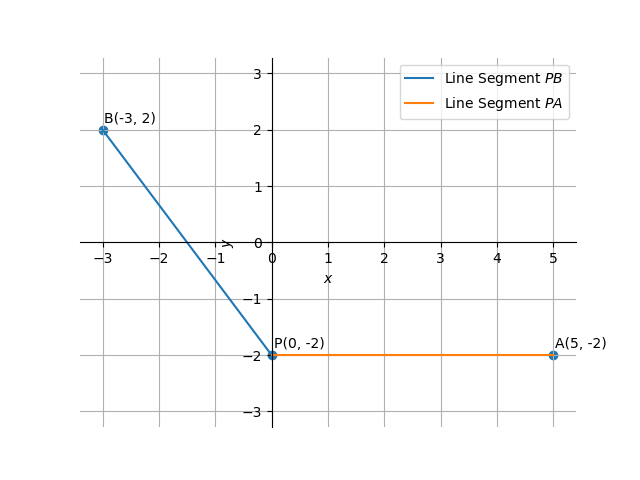
\includegraphics[width=\columnwidth, height=0.8\textheight, keepaspectratio]{Figs/plot(py+C).png}     
\end{frame}

%-------End of Python+C-------------


\begin{frame}[fragile]
    \frametitle{Python Code}
    \begin{lstlisting}
import sys
import math
sys.path.insert(0, '/home/sai-sreevallabh/Matrix_Theory/Matgeo/codes/CoordGeo')
import numpy as np
import matplotlib.image as mpimg
import matplotlib.pyplot as plt
import numpy.linalg as LA

#local imports
from line.funcs import *
from triangle.funcs import *

#if using termux
import subprocess
import shlex

\end{lstlisting}
\end{frame}

\begin{frame}[fragile]
    \frametitle{Python Code}
    \begin{lstlisting}
A = np.array([5,-2]).reshape(-1,1)
B = np.array([-3,2]).reshape(-1,1)
e_2 = np.array([0,1]).reshape(-1,1)

y = (LA.norm(A)*LA.norm(A) - LA.norm(B)*LA.norm(B))/(2*(A-B).T@e_2)

y = y.item()

P = np.array([0,y]).reshape(-1,1)

x_AP = line_gen(A,P)
x_PB = line_gen(P,B)

\end{lstlisting}
\end{frame}

\begin{frame}[fragile]
    \frametitle{Python Code}
    \begin{lstlisting}
plt.plot(x_AP[0,:],x_AP[1,:],label='Line Segment $PA$')
plt.plot(x_PB[0,:],x_PB[1,:],label='Line Segment $PB$')

tri_coords = np.block([[A,B,P]])
plt.scatter(tri_coords[0,:], tri_coords[1,:])
vert_labels = ['A','B','P']
for i, txt in enumerate(vert_labels):
    plt.annotate(f'{txt}\n({tri_coords[0,i]:.0f}, {tri_coords[1,i]:.0f})',
                 (tri_coords[0,i], tri_coords[1,i]), 
                 textcoords="offset points", 
                 xytext=(20,5), 
                 ha='center') 
\end{lstlisting}
\end{frame}

\begin{frame}[fragile]
    \frametitle{Python Code}
    \begin{lstlisting}
ax = plt.gca()
ax.spines['top'].set_color('none')
ax.spines['left'].set_position('zero')
ax.spines['right'].set_color('none')
ax.spines['bottom'].set_position('zero')

plt.legend(loc='best')
plt.grid() 
plt.axis('equal')

plt.savefig("../Figs/plot(py).png")
plt.show()

    \end{lstlisting}
\end{frame}


\begin{frame}{Plot-Using Python only}
    \centering
    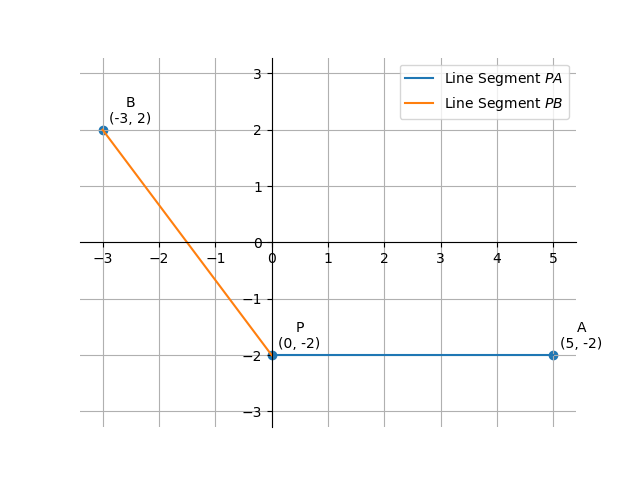
\includegraphics[width=\columnwidth, height=0.8\textheight, keepaspectratio]{Figs/plot(py).png}     
\end{frame}


\end{document}
